
\documentclass[10pt]{article}
\usepackage[margin=1in]{geometry}
\usepackage{amsmath}
\usepackage{amssymb}
\usepackage{setspace}
\usepackage{graphicx}
\usepackage{caption}
\usepackage{listings}
\usepackage{enumitem}
\usepackage{subfigure}


\begin{document}

\title{ECE 4750 Lab 5: Multicore Processor}
\author{Avinash Navada (abn44) \& Akshay Dongaonkar (akd54) 
		\& Vivek Gaddam (vrg22)}
\maketitle


\section{Introduction}

Modern computing applications are increasingly calculation-intensive, highlighting the 
need for systems capable of parallelizing work over multiple execution cores to keep 
total program execution time reasonably low. However, such systems come with
added complexity, and their success relies on design choices, such as the particular
cache and on-chip interconnect network schemes to use. \par

In this lab, we seek to analyze the benefits of using a quad-core system with
a banked data cache and private instruction caches over a single-core system with a data
and instruction cache by comparing their performance on a set of serial and parallel microbenchmarks.
In doing so, we can gain insight into the specific area, energy, and performance tradeoffs between these setups
and draw conclusions on when one system might be more appropriate than the other.

The baseline design is the single-core setup, and the alternative design is the quad-core setup.
In completing both designs, we ultimately found that in terms of total number of cycles per program, multithreaded microbenchmarks run on the alternative design performed better than did single-threaded versions of the same benchmarks run on the baseline.
% INSERT QUANTITATIVE RESULTS HERE!!!! in terms of the number of cycles executed
% INSERT EFFECT OF ALT ON AREA, ENERGY, CYCLE TIME
Based on these results, we can say that we generally expect ...



\section{Project Management}

% 
For this lab, all testing was provided. Therefore, we split the remainder of the work amongst ourselves as follows:
-Avinash wrote the RTL code for the baseline and alternative designs composing the processor cores, caches, and network
-Akshay wrote the version of the quicksort algorithm to be run on the baseline design and parallelized it for testing on the alternative design
-Vivek helped optimize the quicksort C algorithm and was the lead in writing the lab report

Our expected and actual work patterns are shown in Figure~\ref{fig:gantt}.


\section{Baseline Design}

The baseline design for this lab report is a single-core system consisting of a bypassed pipelined PARCv2 
processor, a two-way set-associative instruction cache, and a two-way set-associative data cache. 

Due to an existing bug in our pipelined processor from Lab 2, we decided to use the provided processor core, 
cache, and network units in composing our baseline design. Our design is in accordance with the setup in 
Figure~\ref{fig:bline}. This overall setup is responsible for taking assembly instructions from a provided
instruction memory and interfacing with a provided data memory in order to execute programs.

Because our baseline design is composed entirely of components that were designed in previous labs that were 
tested individually, specifically the caches and processor core, it is a good example of a modular design. 

This design can be viewed as the minimum hardware one expects to have when running full C programs, and is therefore
an appropriate baseline for comparison for more complicated designs, such as the quad-core processor that serves as
our alternative design. Any real system includes caches for instruction and data memories to reduce the average memory
access latency (AMAL), so it makes sense for our baseline implementation to use them as well. 

As part of the requirements of completing the baseline design, we implemented the quicksort algorithm in C for use on
one core. This was used as a microbenchmark in our lab. The provided quicksort method signature contains a ...
A slight optimization that we provided in our lab was to amortize
because this eliminates , this should 

% Diagram of base datapath or block diagram


\section{Alternative Design}

In our alternative design, which is a quad-core system, we use four processor cores identical to the one in the baseline design and compose them with four two-way set-associative instruction caches and four two-way set-associative data caches. Of course, this composition of multiple processor cores and caches must still behave to the outside as a single execution unit that takes instructions from a single instruction memory and uses a single data memory, just as the baseline design does. Therefore, we must coordinate the separate entities with networks. We have special networks between the caches and their respective memory interface. We also use a third interconnect network for handling data cache requests so that they can be sent to the appropriate bank. See Figure~\ref{fig:alt} for the datapath of our alternative design.

One important feature of the alternative design is to use a single banked data cache. In a typical multithreaded application, threads will provide parallelization by performing significant amounts of calculation on some sort of common state. Two observations come from this: first, that the threads will likely access and modify large numbers of data addresses (ex: while streaming through a large array), and second, that the data is shared amongst the threads, regardless of whether or not the threads are performing the same type of work on that data (i.e., whether or not they are dealing with the same instruction PCs). A banked data cache is a response to both of these observations. Given some fixed technology constraints such as a restriction on area devoted to caches, we would like to use the data caches as effectively as possible. Therefore, we would like to share the allowed cache space amongst all threads (to make the cache as big as possible), allowing any particular data address to live in only one place in the shared cache at a time. We do not however bank the instruction caches here; we decide not to always pay the overhead of having a network arbitrate a single banked instruction cache over multiple execution cores when in fact having a banked instruction cache does not necessarily make sense for multithreaded applications.

In some ways, the quicksort application we implement in this lab does not fit this above profile of a multithreaded program. Each thread executes identical instructions (with respect to IPC) but may in fact modify completely disjoint parts of the input array. Nevertheless, we may not typically have such fine parallelization. Furthermore, notice that a single thread is likely to use many different data addresses much quicker than it does distinct instruction PCs in a given timeslice in a typical scenario like looping over a large array. Therefore, even if there are duplicate entries across the private instruction caches, they are likely to live there for many cycles. As always, we try to optimize some scenarios over others while still providing functionality over a wide array of uses.

We would like to see how close our alternative design can come to actually realizing the ideal performance benefit of having four cores with the knowledge that the additional network infrastructure required to make such a design work comes with some energy and performance cost.


\section{Testing Strategy}

As mentioned earlier, the testing suite for this lab was provided to us and consisted of single-threaded source/sink based tests as well as single and multi-threaded self-checking assembly tests. The source/sink tests comprehensively test all PARC v2 instructions compiled for the PARC ISA. Both our baseline and alternative designs passed all tests and benchmarks. 



\section{Evaluation}

Base
----
vvadd:     2294 cyc, 502 instr, 4.57 cpi
cmplx-mult: 9080, 1972, 4.6
bin search: 12205, 2658, 4.59
masked filter: 25596, 5742, 4.46
quicksort: -----

Alt
----
vvadd:     1812 cyc, 233 instr, 7.78 cpi
cmplx-mult: 5525, 641, 8.62
bin search: 6187, 926, 6.68
masked filter: 12827, 1992, 6.44
quicksort: -----


\newpage
\section {Tables and Diagrams}

% Figure: Gantt Chart
% \begin{figure}[h]
% 	\centering
% 	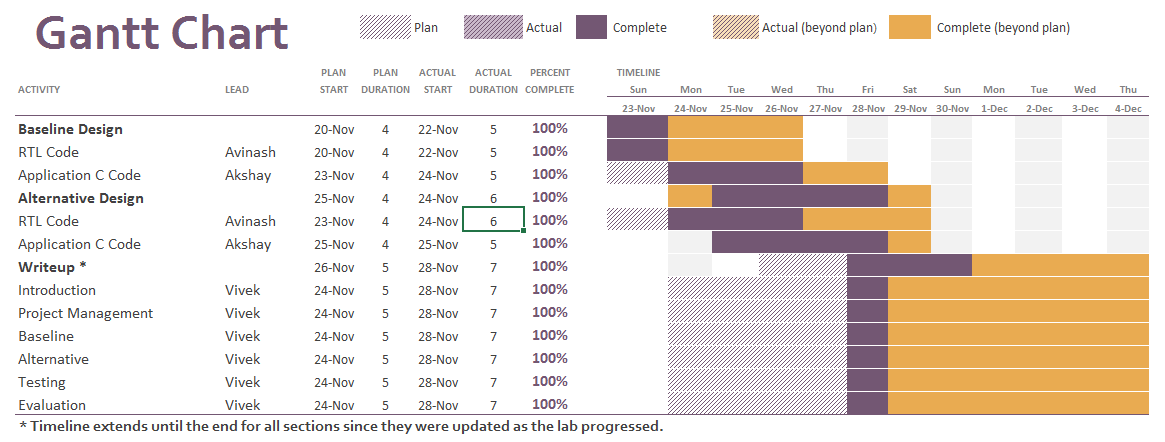
\includegraphics[scale=0.4, angle=90]{gantt}
% 	\caption{Gantt Chart.}
% 	\label{fig:gantt}
% \end{figure}

% Figure: Baseline Design
\begin{figure}[h]
	\centering
	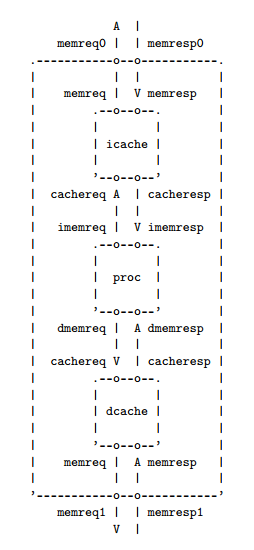
\includegraphics[scale=0.4, angle=90]{bline-diag}
	\caption{Baseline Design - Single-Core system}
\end{figure}

% Figure: Alt Design
\begin{figure}[h]
	\centering
	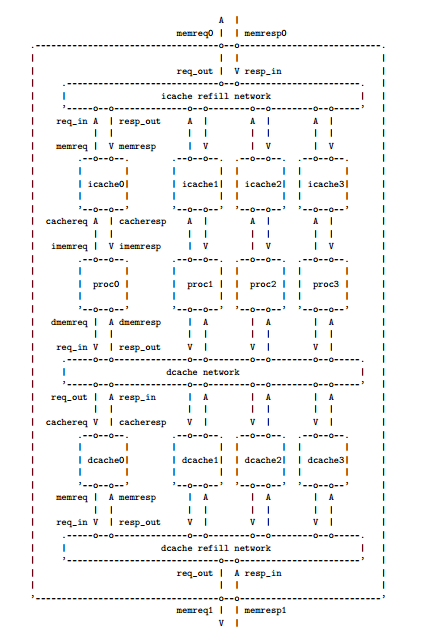
\includegraphics[scale=0.4, angle=90]{alt-diag}
	\caption{Alternative Design - Multi-Core system}
\end{figure}



% END
\end{document}






